
% This LaTeX was auto-generated from MATLAB code.
% To make changes, update the MATLAB code and republish this document.

\documentclass{article}
\usepackage{graphicx}
\usepackage{color}

\sloppy
\definecolor{lightgray}{gray}{0.5}
\setlength{\parindent}{0pt}

\begin{document}

    
    

\section*{10. Best approximation}

\begin{verbatim}
ATAPformats
\end{verbatim}
\begin{par}
An old idea, going back to Chebyshev himself and earlier to Poncelet, is to look for a polynomial $p^*$ of specified degree $n$ that is the \textit{best approximation} to a given continuous function $f$ in the sense of minimizing the $\infty$-norm of the difference  on an interval [Poncelet 1835, Chebyshev 1854 \& 1859]. (A best approximation is also called a \textit{Chebyshev approximation,} but we shall avoid this usage to minimize confusion.  Other terms for the same idea include \textit{minimax} and \textit{equiripple.}) It is known that $p^*$ exists and is unique, as we shall prove below.  There is a Chebfun command \texttt{remez} for computing these approximants, due to Ricardo $\hbox{Pach\'on}$: if $f$ is a chebfun, then \texttt{remez(f,n)} is the chebfun corresponding to its best approximation of degree $n$. For details see $\hbox{[Pach\'on}$ \& Trefethen 2009].
\end{par} \vspace{1em}
\begin{par}
We shall argue in Chapter 16 that best approximations in the $\infty$-norm are not always as useful as one might imagine; Chebyshev interpolants are often as good or even better.  Nevertheless, they represent an elegant and fundamental idea and a line of investigation going back more than 150 years.  So for the moment, let us enjoy them.
\end{par} \vspace{1em}
\begin{par}
For example, here are the best approximants of degree 2 and 4 to $|x|$, together with their \textit{error curves} $(f-p^*)([-1,1])$:
\end{par} \vspace{1em}
\begin{par}
 \vskip -2em 
\end{par} \vspace{1em}
\begin{verbatim}
x = chebfun('x'); f = abs(x);
for n = 2:2:4
  subplot(1,2,1), hold off, plot(f,'k'), grid on
  [p,err] = remez(f,n); hold on, plot(p,'b'), axis([-1 1 -.2 1.2])
  FS = 'fontsize';
  title(['Function and best approx, n = ' int2str(n)],FS,9)
  subplot(1,2,2), hold off, plot(f-p), grid on, hold on
  axis([-1 1 -.15 .15]), title('Error curve',FS,9)
  plot([-1 1],err*[1 1],'--k'), plot([-1 1],-err*[1 1],'--k')
  snapnow
end
\end{verbatim}

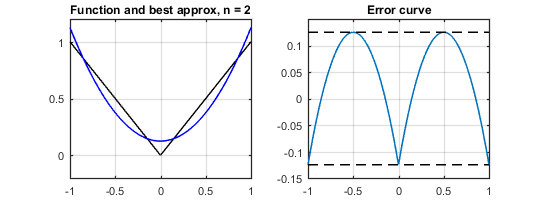
\includegraphics [width=4in]{chap10_01.png}

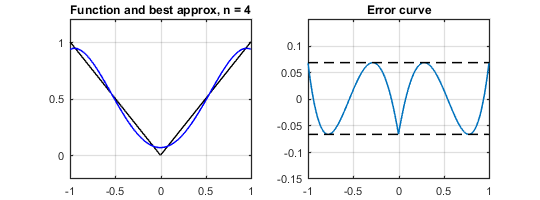
\includegraphics [width=4in]{chap10_02.png}
\begin{par}
 \vskip 1pt 
\end{par} \vspace{1em}
\begin{par}

Notice the {\em equioscillation} property: the error curve attains its
extreme magnitude with alternating signs at a succession of values of
$x$. Chebyshev appears to have known this in the 1850s, and indeed
suggested he was not the first to know it (``comme on le sait'', p.~114
of [Chebyshev 1854]), but he did not explicitly address questions of
existence, uniqueness, or even alternation of signs. More systematic
treatments came at the beginning of the 20th century with work by
Blichfeldt [1901], Kirchberger [1902], and Borel [1905].  It seems to
have been Kirchberger, in his PhD thesis written under Hilbert, who first
stated and proved the characterization theorem that is now so well known
[Kirchberger 1902], proving in particular that a best approximation $p^*$
exists. Note that in the characterization part of this theorem, $f$ is
assumed to be real, whereas most of the discussion in this book allows
$f$ to be real or complex. Existence and uniqueness in the complex case
were established by Tonelli [1908]. Complex generalizations of the
characterization originate with [Kolmogorov 1948] and [Remez 1951]. Many
further generalizations can also be found in the approximation theory
literature, for example with the set of polynomials on an interval
replaced by a more general set of functions satisfying a property known
as the {\em Haar condition.}

\end{par} \vspace{1em}
\begin{par}
\textbf{Theorem 10.1. Equioscillation characterization of best approximants.} \textit{A continuous function $f$ on $[-1,1]$ has a unique best approximation $p^* \in {\cal P}_n$.  If $f$ is real, then $p^*$ is real too, and in this case a polynomial $p\in {\cal P}_n$ is equal to $p^*$ if and only if $f-p$ equioscillates in at least $n+2$ extreme points.}
\end{par} \vspace{1em}
\begin{par}
\textit{Proof.}  A set of $n+2$ points of equioscillation of this kind is called an \textit{alternant,} though we shall not make much use of this term.
\end{par} \vspace{1em}
\begin{par}
To prove existence of a best approximation, we note that $\|f-p\|$ is a continuous function of $p\in {\cal P}_n$.  Since one candidate approximation is the zero function, we know that if $p^*$ exists, it lies in $\{p\in {\cal P}_n: \|f-p\|\le \|f\|\}$. This is a closed and bounded subset of a finite-dimensional space, hence compact (the Bolzano--Weierstrass property), and thus the minimum is attained. (This argument originates with F. Riesz [1918].)
\end{par} \vspace{1em}
\begin{par}
Next we show that equioscillation implies optimality. Suppose $f$ and $p$ are real and $(f-p)(x)$ takes equal extreme values with alternating signs at $n+2$ points $x_0<x_1< \cdots < x_{n+1}$, and suppose $\| f-q\| < \| f-p\|$ for some real polynomial $q\in {\cal P}_n$. Then $p-q$ must take nonzero values with alternating signs at the equioscillation points, implying that it takes the value zero in at least $n+1$ points in-between.  This implies that $p-q$ is identically zero, which is a contradiction.
\end{par} \vspace{1em}
\begin{par}
The third step is to show that optimality implies equioscillation (this part of the argument was given in [Blichfeldt 1901]). Suppose $f-p$ equioscillates at fewer than $n+2$ points, and set $E=\|f-p\|$. Without loss of generality suppose the leftmost extremum is one where $f-p$ takes the value $-E$.  Then there are numbers $-1< x_1< \cdots  < x_k< 1$ with $k\le n$ such that $(f-p)(x) <E$ for $x\in [-1,x_1] \cup [x_2,x_3] \cup [x_4,x_5] \cup \cdots$ and $(f-p)(x)>-E$ for $x\in [x_1,x_2] \cup [x_3,x_4] \cup \cdots.$ If we define $\delta p(x) = (x_1-x)(x_2-x)\cdots (x_k-x)$, then $(\kern .7pt p-\varepsilon \delta p)(x)$ will be a better approximation than $p$ to $f$ for all sufficiently small $\varepsilon>0$.
\end{par} \vspace{1em}
\begin{par}
Finally, to prove uniqueness of best approximations---we treat the real case only---we refine the argument that equioscillation implies optimality.  Suppose $p$ is a best approximation with equioscillation extreme points $x_0<x_1< \cdots < x_{n+1}$, and suppose $\| f-q\| \le \| f-p\|$ for some real polynomial $q\in {\cal P}_n$. Then (without loss of generality) $(\kern .7pt p-q)(x)$ must be $\le 0$ at $x_0, x_2, x_4, \dots$ and $\ge 0$ at $x_1, x_3, x_5, \dots.$  This implies that $p-q$ has roots in each of the $n+1$ closed intervals $[x_0,x_1], [x_1,x_2], \dots ,[x_n,x_{n+1}]$.  We wish to conclude that $p-q$ has at least $n+1$ roots in total, counted with multiplicity, implying that $p=q$.  To make the argument we prove by induction that $p-q$ has at least $k$ roots in $[x_0,x_k]$ for each $k$. The case $k=1$ is immediate. For the general case, suppose $p-q$ has at least $j$ roots in $[x_0,x_j]$ for each $j\le k-1$ but only $k-1$ roots in $[x_0,x_k]$. Then there must be a simple root at $x_{k-1}$. By the induction hypothesis, $p-q$ must have exactly $k-2$ roots in $[x_0,x_{k-2}]$ with a simple root at $x_{k-2}$, $k-3$ roots in $[x_0,x_{k-3}]$ with a simple root at $x_{k-3}$, and so on down to $1$ root in $[x_0,x_1]$, with a simple root at $x_1$. It follows that $p-q$ must be nonzero at $x_0$ and at $x_k$, and since the sign of $p-q$ changes at each of the simple roots $x_1,\dots x_{k-1}$, the signs at $x_0$ and $x_k$ must be the same if $k$ is odd and opposite if $k$ is even.  On the other hand from the original alternation condition we know that $p-q$ must take the same signs at $x_0$ and $x_k$ if $k$ is even and opposite signs if $k$ is odd.
\end{par} \vspace{1em}
\begin{par}
There is a simpler proof of uniqueness than the one just given, in which one supposes $p$ and $q$ are distinct best approximations and considers $(\kern .7pt p+q)/2$ (Exercise 10.10).  However, that proof does not generalize to the problem of rational approximation (Theorem 24.1). $~\hbox{\vrule width 2.5pt depth 2.5 pt height 3.5 pt}$
\end{par} \vspace{1em}
\begin{par}
Note that the error curve for a best approximation may have more than $n+2$ points of equioscillation, and indeed this will always happen if $f$ and $n$ are both even or both odd (Exercise 10.4).  For example, for the function $f(x) = |x|$ considered above, the degree 2 approximation equioscillates at 5 points, not 4, and the degree 4 approximation equioscillates at 7 points, not 6. This phenomenon of ``extra'' points of equioscillation will become important in the generalization to rational approximation in Chapter 24.
\end{par} \vspace{1em}
\begin{par}
Here is another example, the degree 10 best approximation to $\exp(x)$. There are 12 points of equioscillation.
\end{par} \vspace{1em}
\begin{par}
 \vskip -2em 
\end{par} \vspace{1em}
\begin{verbatim}
f = exp(x);
[p,err] = remez(f,10);
clf, plot(f-p), grid on, hold on
title('Error curve, degree 10',FS,9)
plot([-1 1],err*[1 1],'--k'), plot([-1 1],-err*[1 1],'--k')
\end{verbatim}

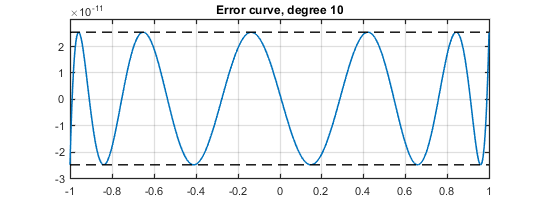
\includegraphics [width=4in]{chap10_03.png}
\begin{par}
 \vskip 1pt 
\end{par} \vspace{1em}
\begin{par}
And here is another example.  The Chebfun \texttt{cumsum} command returns the indefinite integral, producing in this case a zigzag function.
\end{par} \vspace{1em}
\begin{par}
 \vskip -2em 
\end{par} \vspace{1em}
\begin{verbatim}
f = cumsum(sign(sin(20*exp(x))));
clf, plot(f,'k'), hold on
[p,err] = remez(f,20);
plot(p), grid on, title('Function and best approximation',FS,9)
\end{verbatim}

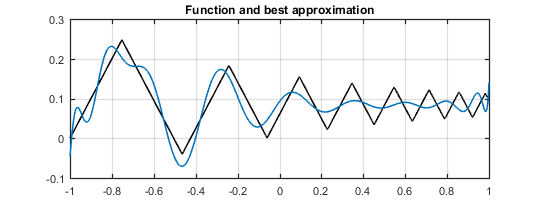
\includegraphics [width=4in]{chap10_04.png}
\begin{par}
 \vskip 1pt 
\end{par} \vspace{1em}
\begin{par}
The corresponding error curve reveals $20+2=22$ points of equioscillation:
\end{par} \vspace{1em}
\begin{par}
 \vskip -2em 
\end{par} \vspace{1em}
\begin{verbatim}
hold off, plot(f-p), grid on, hold on, axis([-1 1 -.06 .06])
plot([-1 1],err*[1 1],'--k'), plot([-1 1],-err*[1 1],'--k')
title('Error curve, degree 20',FS,9)
\end{verbatim}

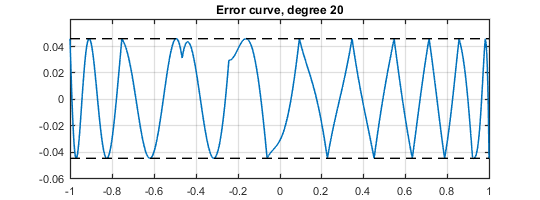
\includegraphics [width=4in]{chap10_05.png}
\begin{par}
 \vskip 1pt 
\end{par} \vspace{1em}
\begin{par}
Here's the analogous curve for degree 30, plotted on the same scale.
\end{par} \vspace{1em}
\begin{par}
 \vskip -2em 
\end{par} \vspace{1em}
\begin{verbatim}
[p,err] = remez(f,30);
hold off, plot(f-p), grid on, hold on, axis([-1 1 -.06 .06])
plot([-1 1],err*[1 1],'--k'), plot([-1 1],-err*[1 1],'--k')
title('Error curve, degree 30',FS,9)
\end{verbatim}

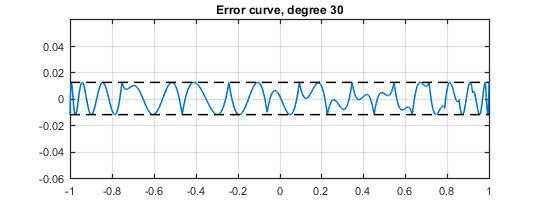
\includegraphics [width=4in]{chap10_06.png}
\begin{par}
 \vskip 1pt 
\end{par} \vspace{1em}
\begin{par}
The algorithm underlying \texttt{remez}, known as the \textit{Remez algorithm} or the \textit{exchange algorithm,} goes back to the Soviet mathematician Evgeny Remez in 1934, and is based on iteratively adjusting a trial alternant until it converges to a correct one [Remez 1934a, 1934b, 1957; Powell 1981]. We shall not give details here, but in fact, Chebfun is an excellent platform for such computations since the algorithm depends on repeatedly finding the local extrema of trial error curves, an operation carried out easily via the \texttt{roots} command (see Chapter 18). Also crucial to the success of \texttt{remez} is the use of the barycentric representation (5.11) for all polynomials, based not at Chebyshev points but at the points of each trial alternant $\hbox{[Pach\'on}$ \& Trefethen 2009].  (The observations of [Webb, Gonnet \& Trefethen 2011] suggest that it might be better to use the ``first barycentric formula'' (5.9).)
\end{par} \vspace{1em}
\begin{par}
The history of the Remez algorithm is interesting, or perhaps we should say the sociology.  It stands out as one of the preeminent examples of a nontrivial algorithm for a nonlinear computational problem that was developed before the invention of computers.  Perhaps in part because of this early appearance, it became remarkably well known, a fixture in numerical analysis courses worldwide.  One might imagine, based on its fame, that the Remez algorithm must be very important in practice, but in fact it seems there is not much software and just a moderate amount of use of these ideas.  One application has been in the design of routines for computing special functions [Cody, Fraser \& Hart 1968, Cody 1993, Muller 2006].  Another is in the field of digital signal processing, where variants of the Remez ideas were developed by Parks and McClellan beginning in 1971 with tremendous success for designing low-pass, high-pass, and other digital filters [Parks \& McClellan 1972]. Parks and McClellan too found that the use of a barycentric representation was crucial, as they describe memorably in [McClellan \& Parks 2005].
\end{par} \vspace{1em}
\begin{par}
Chapter 16 will show that Chebyshev interpolants are often as good as best approximations in practice, and this fact may have something to do with why the Remez algorithm is used rather little.  Chapter 20 will show that if you really want a best approximation, it may be more practical to compute it by CF approximation than by the Remez algorithm, at least if $f$ is smooth.  There are also other algorithms for computing best approximations, based for example on linear programming, which we shall not discuss.
\end{par} \vspace{1em}
\begin{par}

\begin{displaymath}
\framebox[4.7in][c]{\parbox{4.5in}{\vspace{2pt}\sl
{\sc Summary of Chapter 10.}
Any $f\in C([-1,1])$ has a unique best approximation $p^*\in {\cal P}_n$
with respect to the $\infty$-norm.  If $f$ is real, $p^*$ is
characterized by having an error curve that equioscillates between at
least $n+2$ extreme points.\vspace{2pt}}}
\end{displaymath}

\end{par} \vspace{1em}
\begin{par}
 \small\smallskip\parskip 2pt
{\bf Exercise 10.1.  A function with spikes.}  Compute numerically the
degree $10$ polynomial best approximation to $\hbox{sech}^2(5(x+0.6)) +
\hbox{sech}^4(50(x+0.2)) + \hbox{sech}^6(500(x-0.2))$ on $[-1,1]$ and
plot $f$ together with $p^*$ as well as the error curve.  What is the
error?  How does this compare with the error in 11-point Chebyshev
interpolation?  (For these Chebfun computations to be practical,
use \verb|'splitting','on'|.)
\par
{\bf Exercise 10.2.  Best approximation of \boldmath$|x|$.}  (a) Use
Chebfun to determine the errors $E_n = \|f-p_n\|$ in degree $n$ best
approximation of $f(x) = |x|$ on $[-1,1]$ for $n = 2,4,8, \dots, 256$,
and make a table of the values $\beta_n = nE_n$ as a function of $n$.
(b) Use Richardson extrapolation to improve your data.  How many digits
can you estimate for the limiting number $\beta = \lim_{n\to\infty}
\beta_n$?  (We shall discuss this problem in detail in Chapter~25.)
\par
{\bf Exercise 10.3.}  $\hbox{\bf de la Vall\'ee Poussin lower bound.}$
Suppose an approximation $p\in {\cal P}_n$ to $f\in C([-1,1])$
approximately equioscillates in the sense that there are points $-1\le
s_0< s_1 < \cdots < s_{n+1}\le 1$ at which $f-p$ alternates in sign with
$|f(s_j)-p(s_j)| \ge \varepsilon$ for some $\varepsilon > 0$.  Show that
$\|f-p^*\|\ge \varepsilon$.  (This estimate originates in [de la Vall\'ee
Poussin 1910].)
\par
{\bf Exercise 10.4.  Best approximation of even functions.} Let $f\in
C([-1,1])$ be an even function, i.e., $f(-x) = f(x)$ for all $x$.  (a)
Prove as a corollary of Theorem 10.1 that for any $n\ge 0$, the best
approximation $p_n^*$ is even.
(b) Prove that for any $n\ge 0$, $p_{2n}^* = p_{2n+1}^*$.
(c) Conversely, suppose $f\in C([-1,1])$ is not even.
Prove that for all sufficiently large $n$, its
best approximations $p_n^*$ are not even.
\par
{\bf Exercise 10.5.  An invalid theorem.} The first two figures of this
chapter suggest the following ``theorem'': {\em if $f$ is an even
function on $[-1,1]$ and $p^*$ is its best approximation of some degree
$n$, then one of the extreme points of $|(f-p^*)(x)|$ occurs at $x=0$.}
Pinpoint the flaw in the following ``proof''.  By the argument of
Exercise 10.4(b), $p^*$ is the best approximation to $f$ for all $n$ in
some range of the form $\hbox{even}\le n \le \hbox{odd}$, such as $4\le n
\le 5$ or $10\le n \le 13$. By Theorem 10.1, the number of
equioscillation points of $f-p^*$ must accordingly be of the form
$\hbox{odd} + 2$, that is, odd.  By symmetry, $0$ must be one of these
points.
\par
{\bf Exercise 10.6.  Nonlinearity of best approximation operator.} We
have mentioned that for given $n$, the operator that maps a function
$f\in C([-1,1])$ to its best degree $n$ approximation $p_n^*$ is nonlinear.
Prove this (on paper, not numerically) by finding two functions $f_1$ and
$f_2$ and an integer $n\ge 0$ such that the best approximation of the sum
in ${\cal P}_n$ is not the sum of the best approximations.
\par
{\bf Exercise 10.7.  Bernstein's lethargy theorem.} Exercise 6.1 considered
a function of Weierstrass, continuous but nowhere differentiable.  A
variant of the same function based on Chebyshev polynomials would be
$$ f(x) = \sum_{k=0}^\infty 2^{-k} T_{3^k}^{}(x). \eqno (10.1) $$
(a) Show that the polynomial
$f_{3^k}^{}$ obtained by truncating (10.1) to degree $3^k$
is the best approximation to $f$ in the spaces ${\cal P}_n$ for certain $n$.
What is the complete set of $n$ for which this is true?  What is the error?
(b) Let $\{\varepsilon_n\}$
be a sequence decreasing monotonically to $0$.  Prove that there is a function
$f\in C([-1,1])$ such that $\|f-p_n^*\|\ge \varepsilon_n$ for all $n$.
(Hint: change the coefficients $2^{-k}$ of (10.1) to values related
to $\{\varepsilon_n\}$.)
\par
{\bf Exercise 10.8.  Continuity of best approximation operator.} For any
$n\ge 0$, the mapping from functions $f\in C([-1,1])$ to their best
approximants $p^*\in {\cal P}_n$ is continuous with respect to the
$\infty$-norm in $C([-1,1])$.  Prove this by an argument combining the
uniqueness of best approximations with compactness.  (This continuity
result appears in Section I.5 of [Kirchberger 1902].
In fact, the mapping is not just
continuous but Lipschitz continuous, a property known as {\em strong
uniqueness,} but this is harder to prove.)
\par
{\bf Exercise 10.9.  Approximation of \boldmath$e^x$.} Truncating the
Taylor series for $e^x$ gives polynomial approximations with maximum
error $E_n \sim 1/(n+1)!$ on $[-1,1]$, but the best approximations do better
by a factor of $2^n$:
$$ E_n \sim {1 \over 2^n (n+1)!}, \quad n\to\infty. \eqno (10.2) $$
(a) Derive (10.2) by combining Exercises 3.15 and 10.3
with the asymptotic formula $I_k(1) \sim 1/(2^n n!)$.
(b) Make a table comparing this estimate with the actual values
$E_n$ computed numerically for $0\le n\le 10$.
\par
{\bf Exercise 10.10.  Alternative proof of uniqueness.}  Prove uniqueness
of the degree $n$ best approximant to a real continuous function $f$ by a
simpler argument than the one given in the proof of Theorem 10.1: suppose
$p$ and $q$ are best approximants, and apply the equioscillation
characterization to $r = (\kern .7pt p+q)/2$.
\par
{\bf Exercise 10.11.  Chebyshev polynomials and best approximations.}
(a) What is the best degree $n$ polynomial approximation to $x^{n+1}$ on $[-1,1]$?
What is the error?  Derive the answers from Theorem~10.1, using the
fact that $T_{n+1}$ oscillates between values $\pm 1$ at $n+2$ points in $[-1,1]$.
(b) What is the best approximation to $0$ among monic polynomials
of degree $n+1$?  What is the error?
\par
{\bf Exercise 10.12.  Every best approximant is an interpolant.}  Let $p$ be the
best approximation in ${\cal P}_n$ to a real function $f\in C([-1,1])$.
Show that there exist $n+1$ distinct points $-1 < x_0 < x_1 < \cdots < x_n < 1$ such
that $p$ is the interpolant in ${\cal P}_n$ to $f$ in the points $\{x_j\}$.
\par
{\bf Exercise 10.13.  A contrast to Faber's theorem.}
Although Faber showed that there does not exist an array of nodes
in $[-1,1]$ whose polynomial interpolants converge for every $f\in C[-1,1]$,
for any {\em fixed} $f$ there exists an array whose
interpolants converge to $f$ [Marcinkiewicz 1936/7].  Prove this by
combining the Weierstrass approximation theorem with the result of the
previous exercise.
\par
{\bf Exercise 10.14.  Asymptotics of the leading coefficient.}
Let $\{\kern .5pt p_n^*\}$ be the sequence of best approximations of a function
$f\in C([-1,1])$, and let $p_n^*$ have leading Chebyshev coefficient
$a_n^*$.  It is known that $\limsup_{n\to\infty} |a_n^*|^{1/n} \le 1$,
with strict inequality if and only if $f$ is analytic on $[-1,1]$
[Blatt \& Saff 1986, Thm.\ 2.1].  Verify this result numerically by estimating
$\limsup_{n\to\infty} |a_n^*|^{1/n}$ for $f(x) = |x|$ and $f(x) = 1/(1+25x^2)$.
\par 
\end{par} \vspace{1em}



\end{document}
    
